\chapter{Αποτελέσματα}
\label{results}
\chapterprecis{
Το κεφάλαιο των Αποτελεσμάτων μελετά τα δυναμικά χαρακτηριστικά πτερυγισμού \textlatin{(flutter)} του φτερού \textlatin{ASW28}. Επιπλέον, παρουσιάζονται τα αποτελέσματα των τεχνικών βελτιστοποίησης που εφαρμόστηκαν. Τέλος, αποδεικνύεται η δυνατότητα που έχουν τα Νευρωνικά Δίκτυα να προβλέπουν την ταχύτητα πτερυγισμού του φτερού.}


\section{Ανάλυση Ιδιομορφών}
\label{modal-analysis}

Για μια καλύτερη κατανόηση των τρόπων με τους οποίους ταλαντώνεται ή πτέρυγα, πραγματοποιείται μια απλή ανάλυση ιδιομορφών. Οι ιδιομορφές και τα ιδιοδιανύσματα που προκύπτουν από αυτήν την ανάλυση είναι εκείνα που θα προέκυπταν σε μια ανάλυση πτερυγιμού για μηδενική ταχύτητα αέρα. Οι πρώτες 6 ιδιομορφές του φτερού παρουσιάζονται στο \autoref{fig:asw28modes}:


\begin{figure}[H]
  \centering
  \subfloat[\textlatin{Mode 1},\quad $f = 1.518 Hz$]{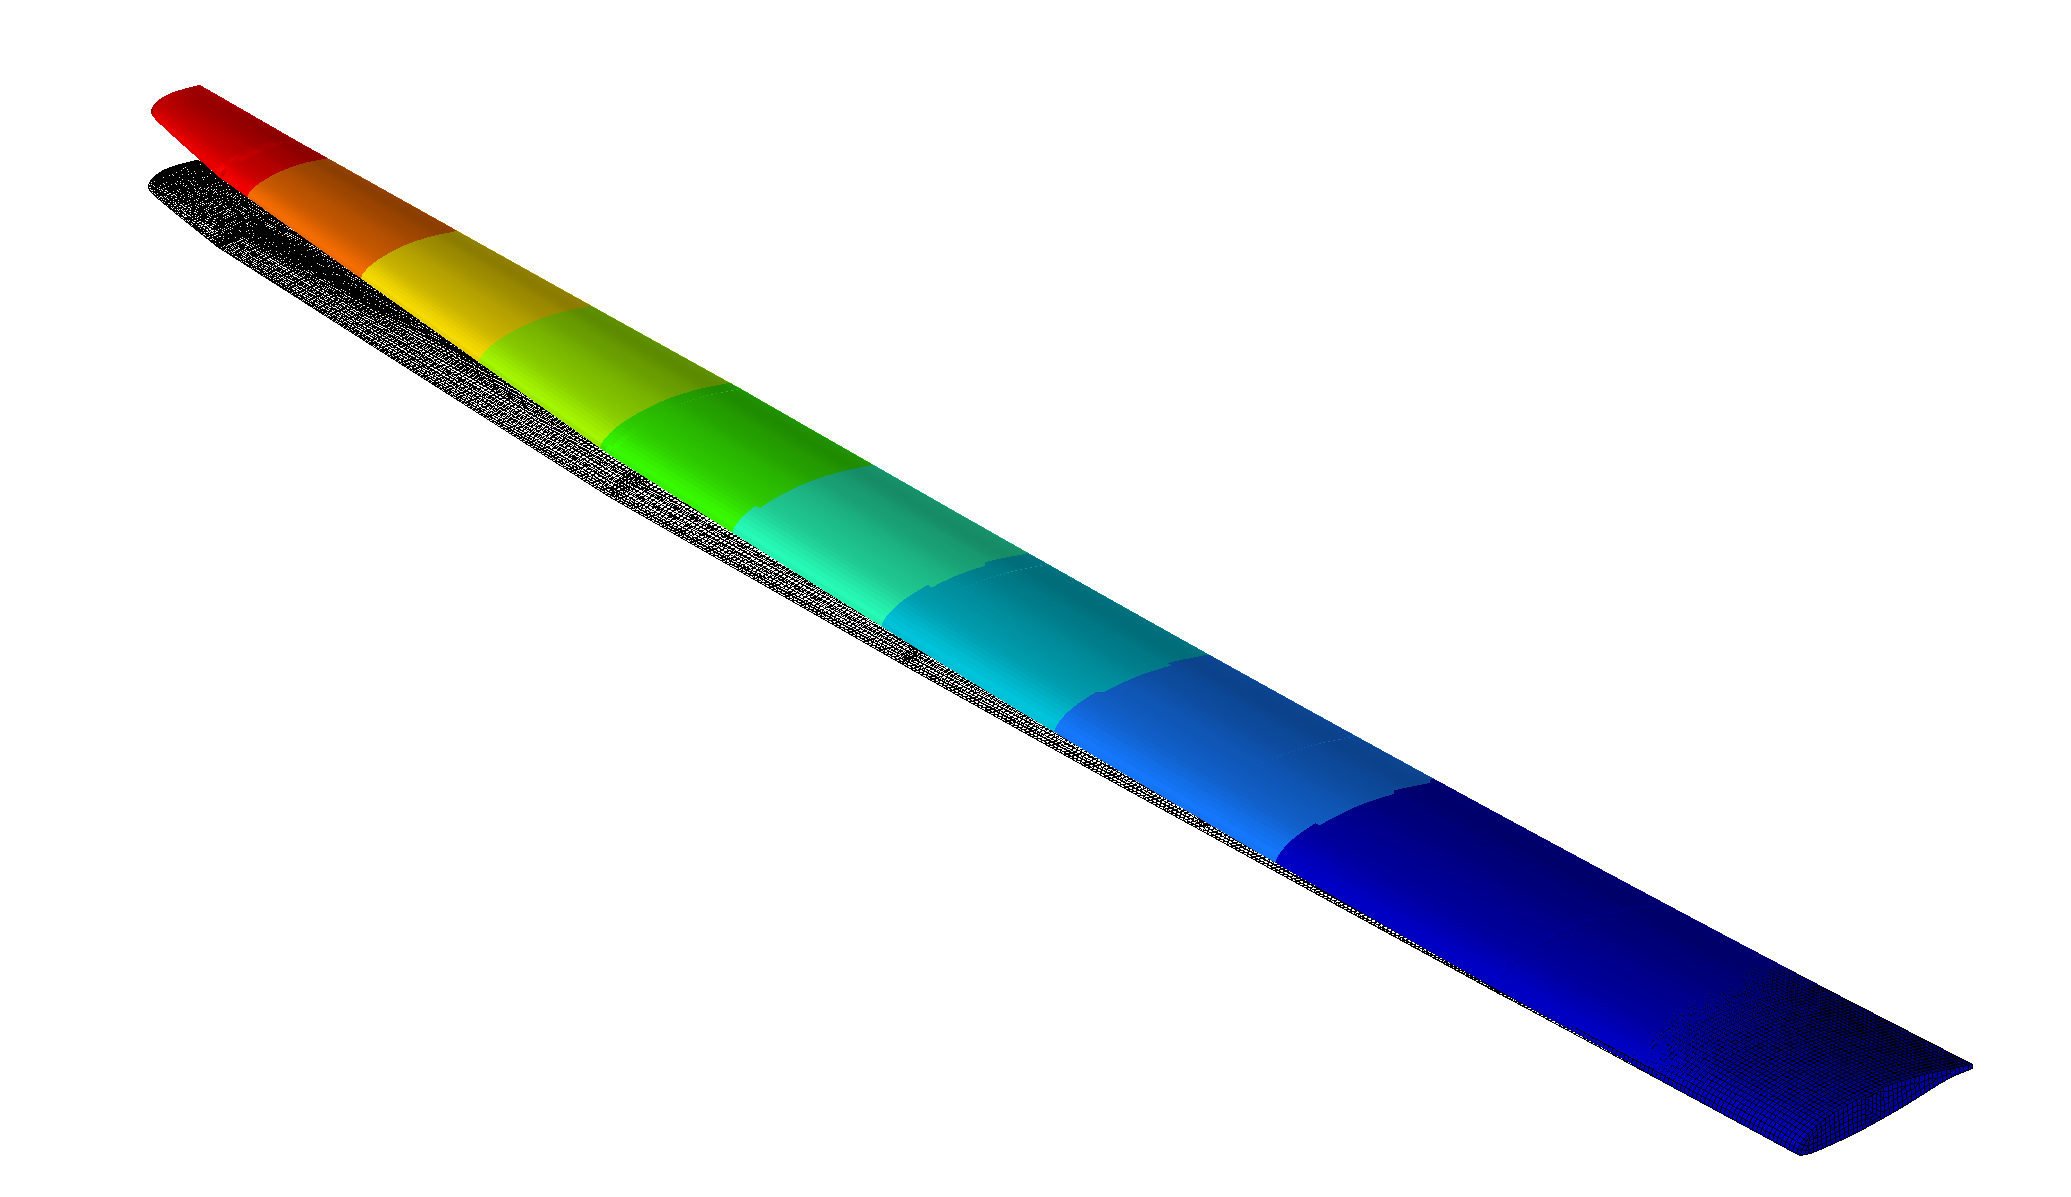
\includegraphics[width=0.5\textwidth]{mode1_1.518Hz.png}}
  \subfloat[\textlatin{Mode 2},\quad $f = 2.704 Hz$]{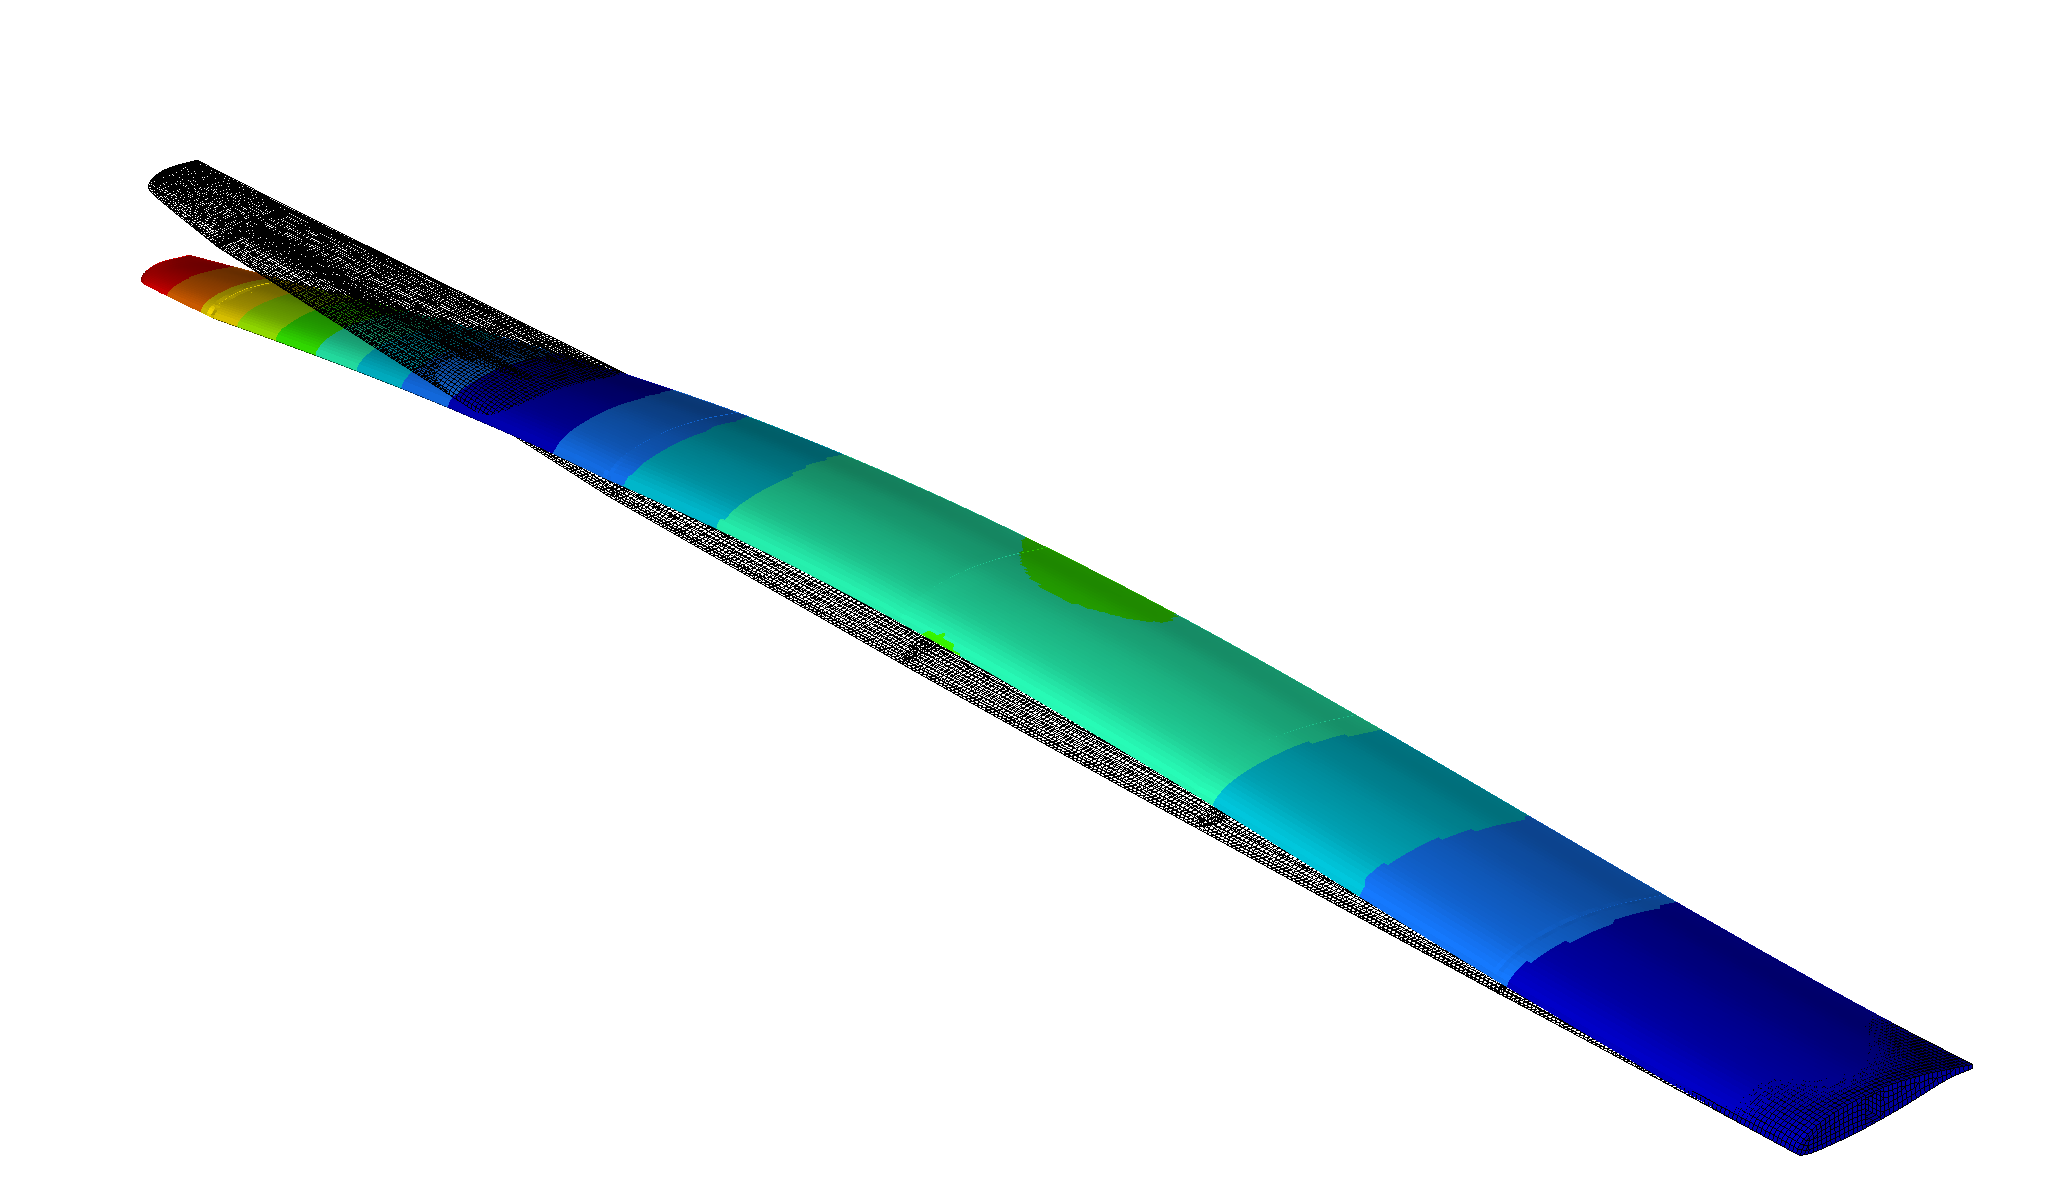
\includegraphics[width=0.5\textwidth]{mode2_7.042Hz.png}}\\
  \subfloat[\textlatin{Mode 3},\quad $f = 7.061 Hz$]{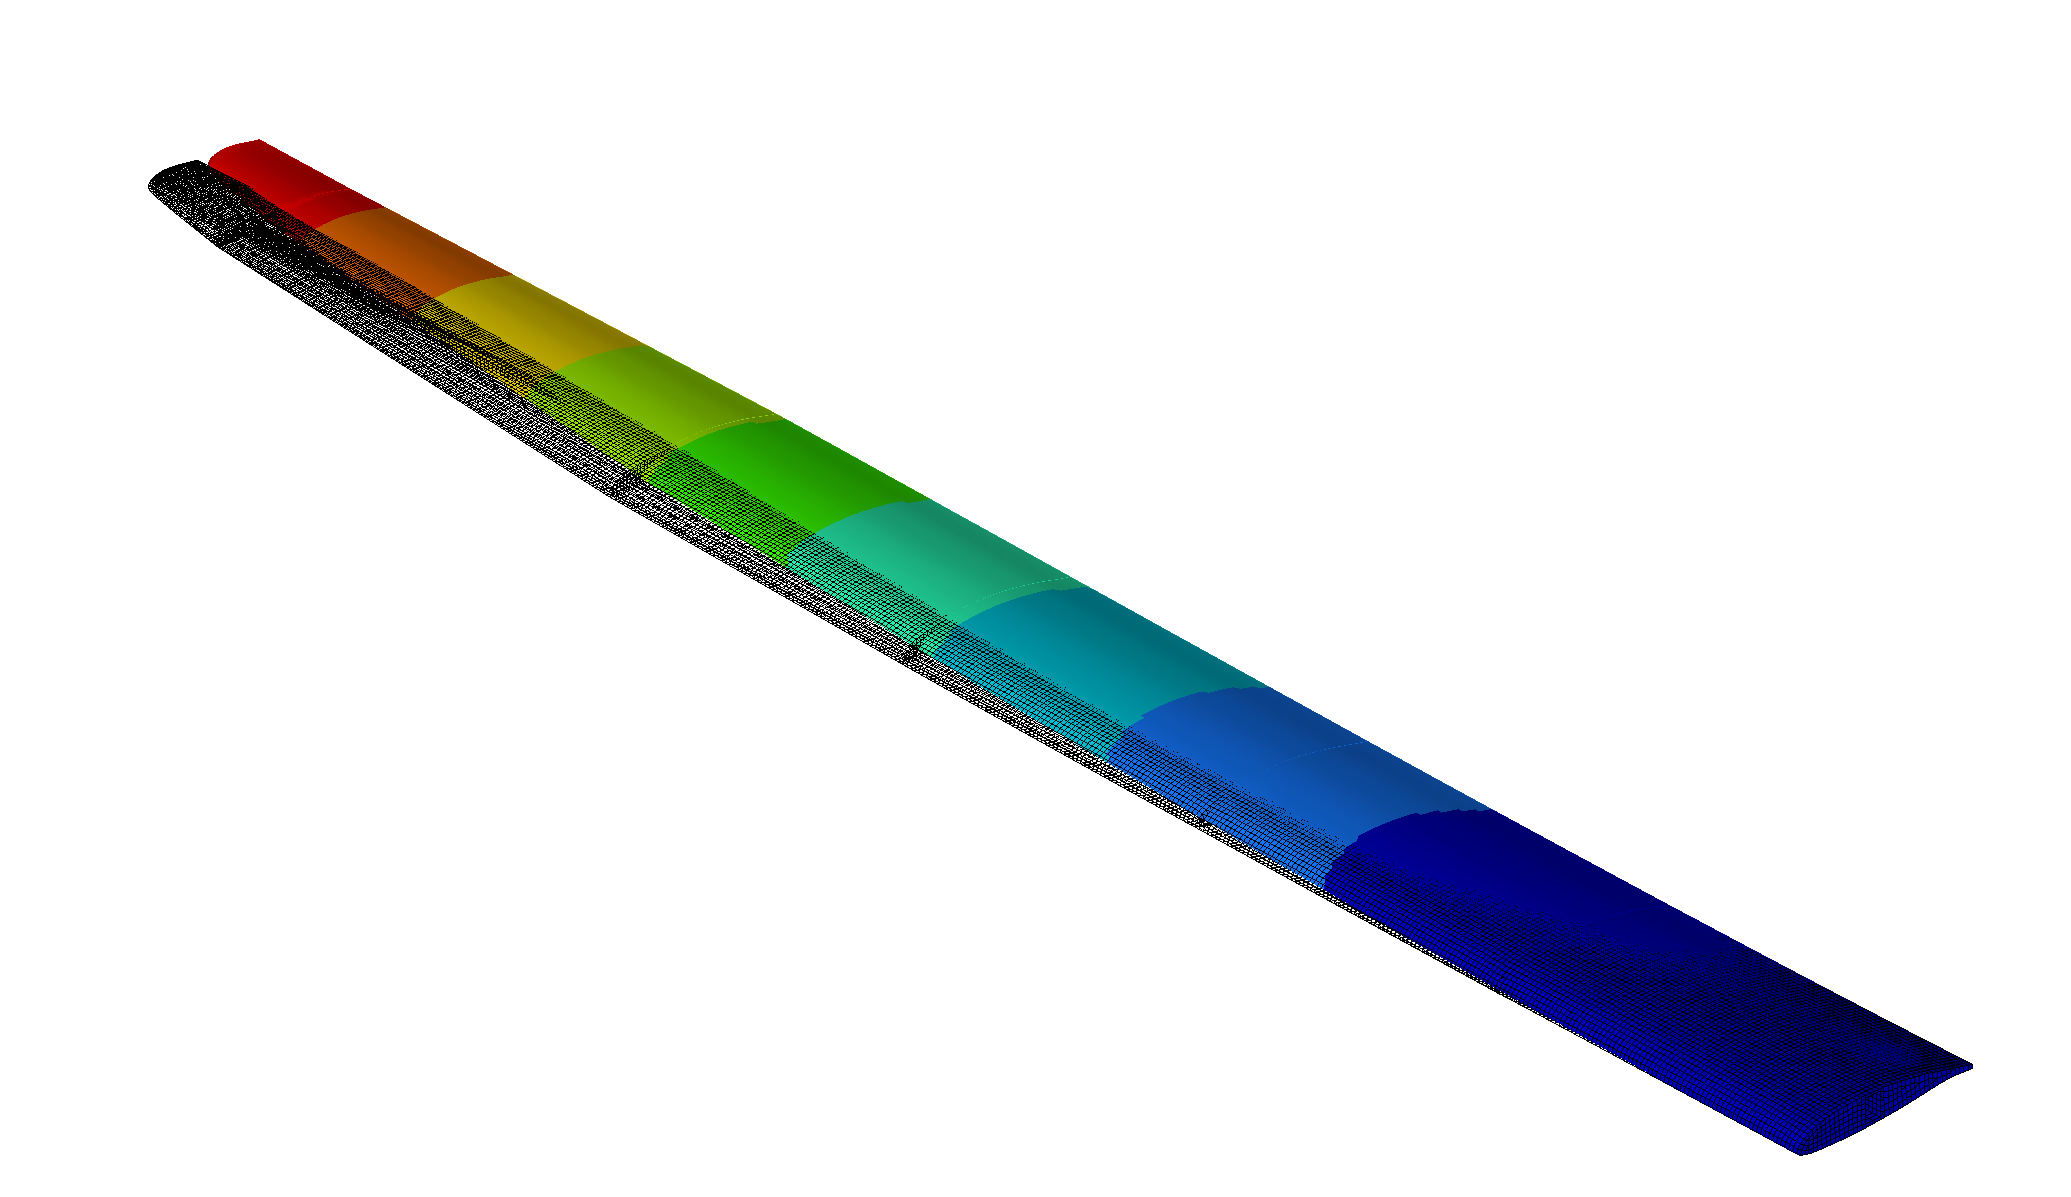
\includegraphics[width=0.5\textwidth]{mode3_7.061Hz.png}} 
  \subfloat[\textlatin{Mode 4},\quad $f = 17.38 Hz$]{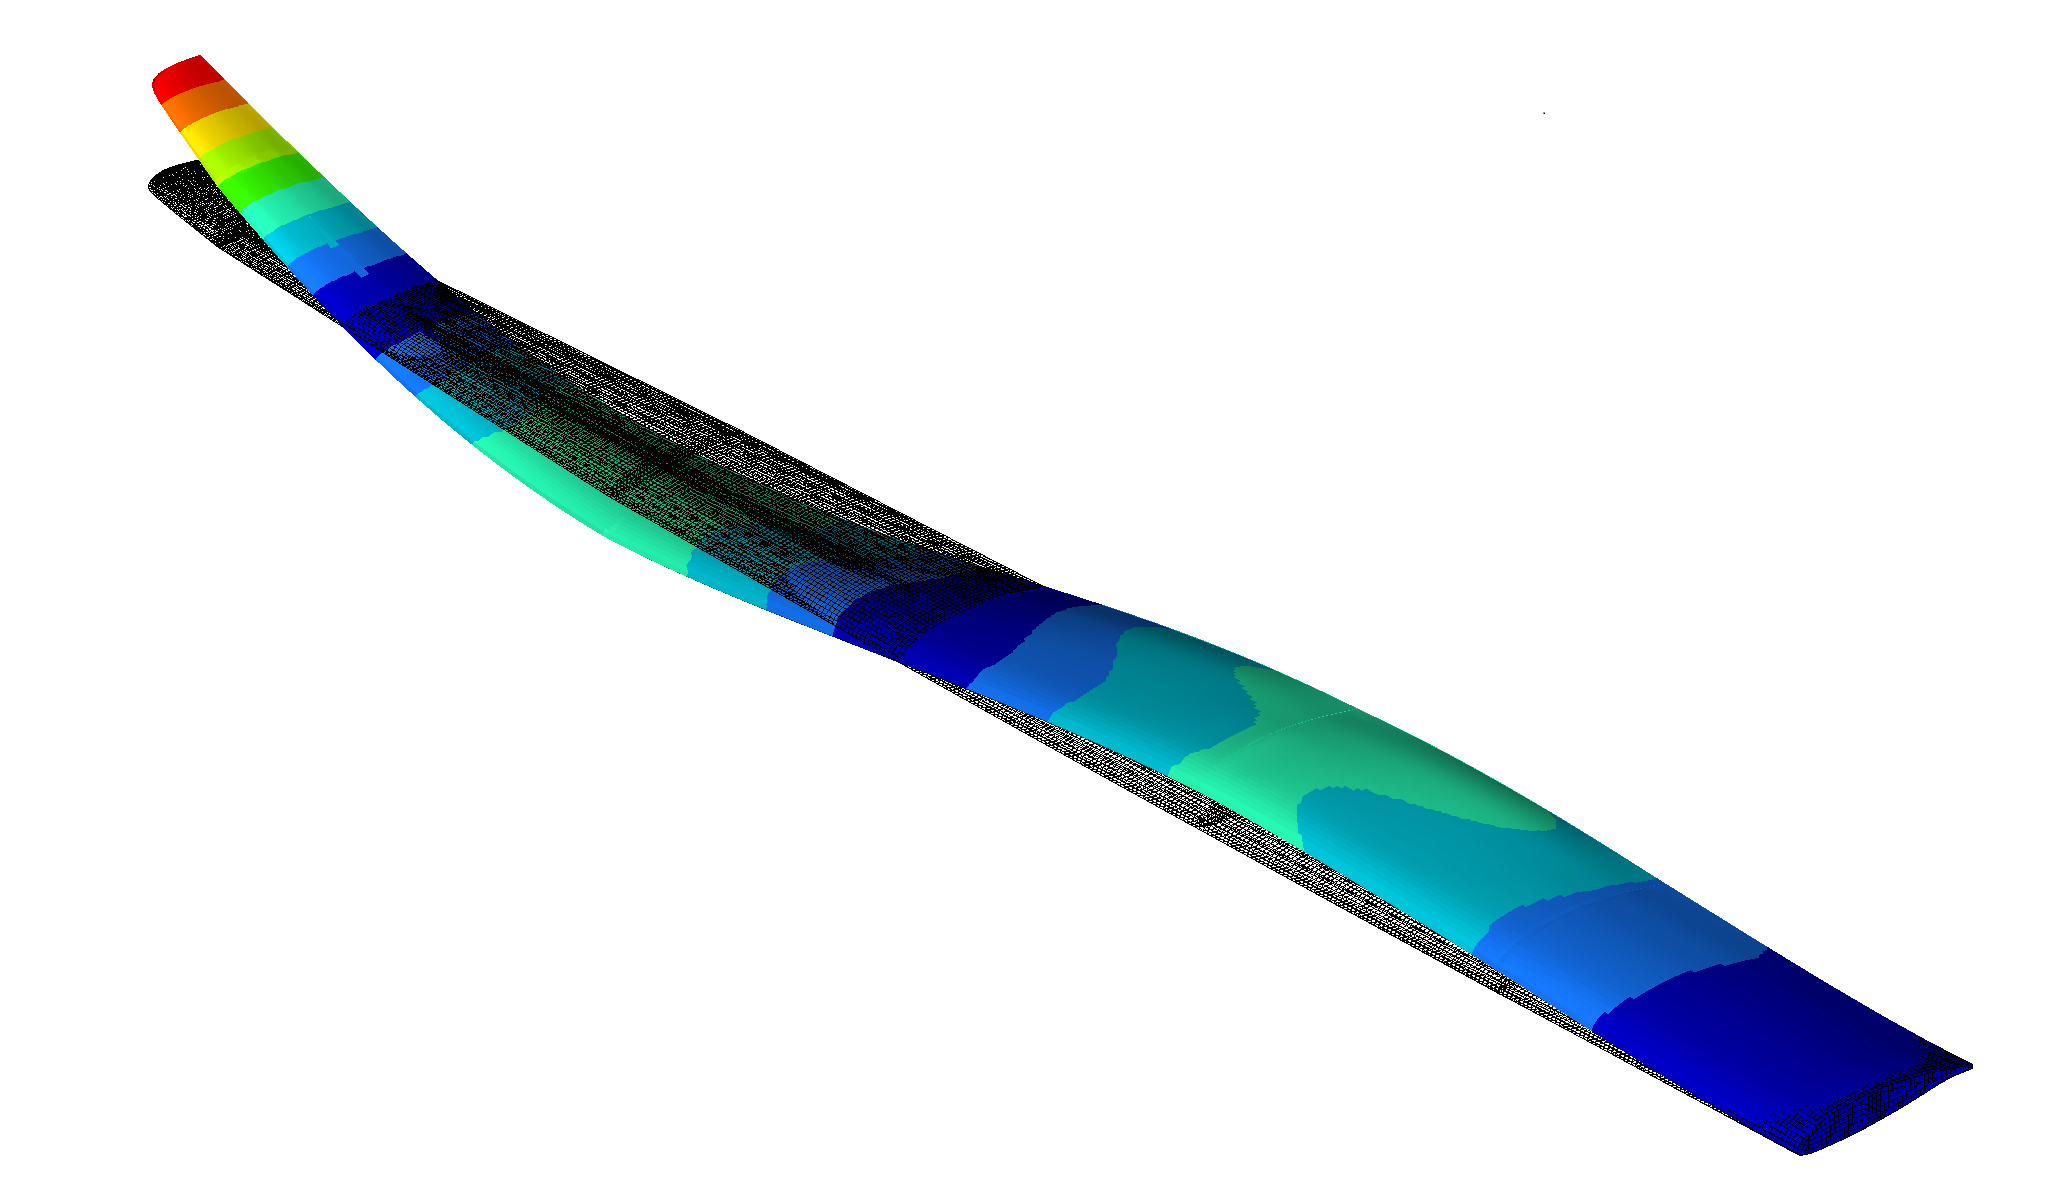
\includegraphics[width=0.5\textwidth]{mode4_17.386Hz.png}}\\
  \subfloat[\textlatin{Mode 5},\quad $f = 30.02 Hz$]{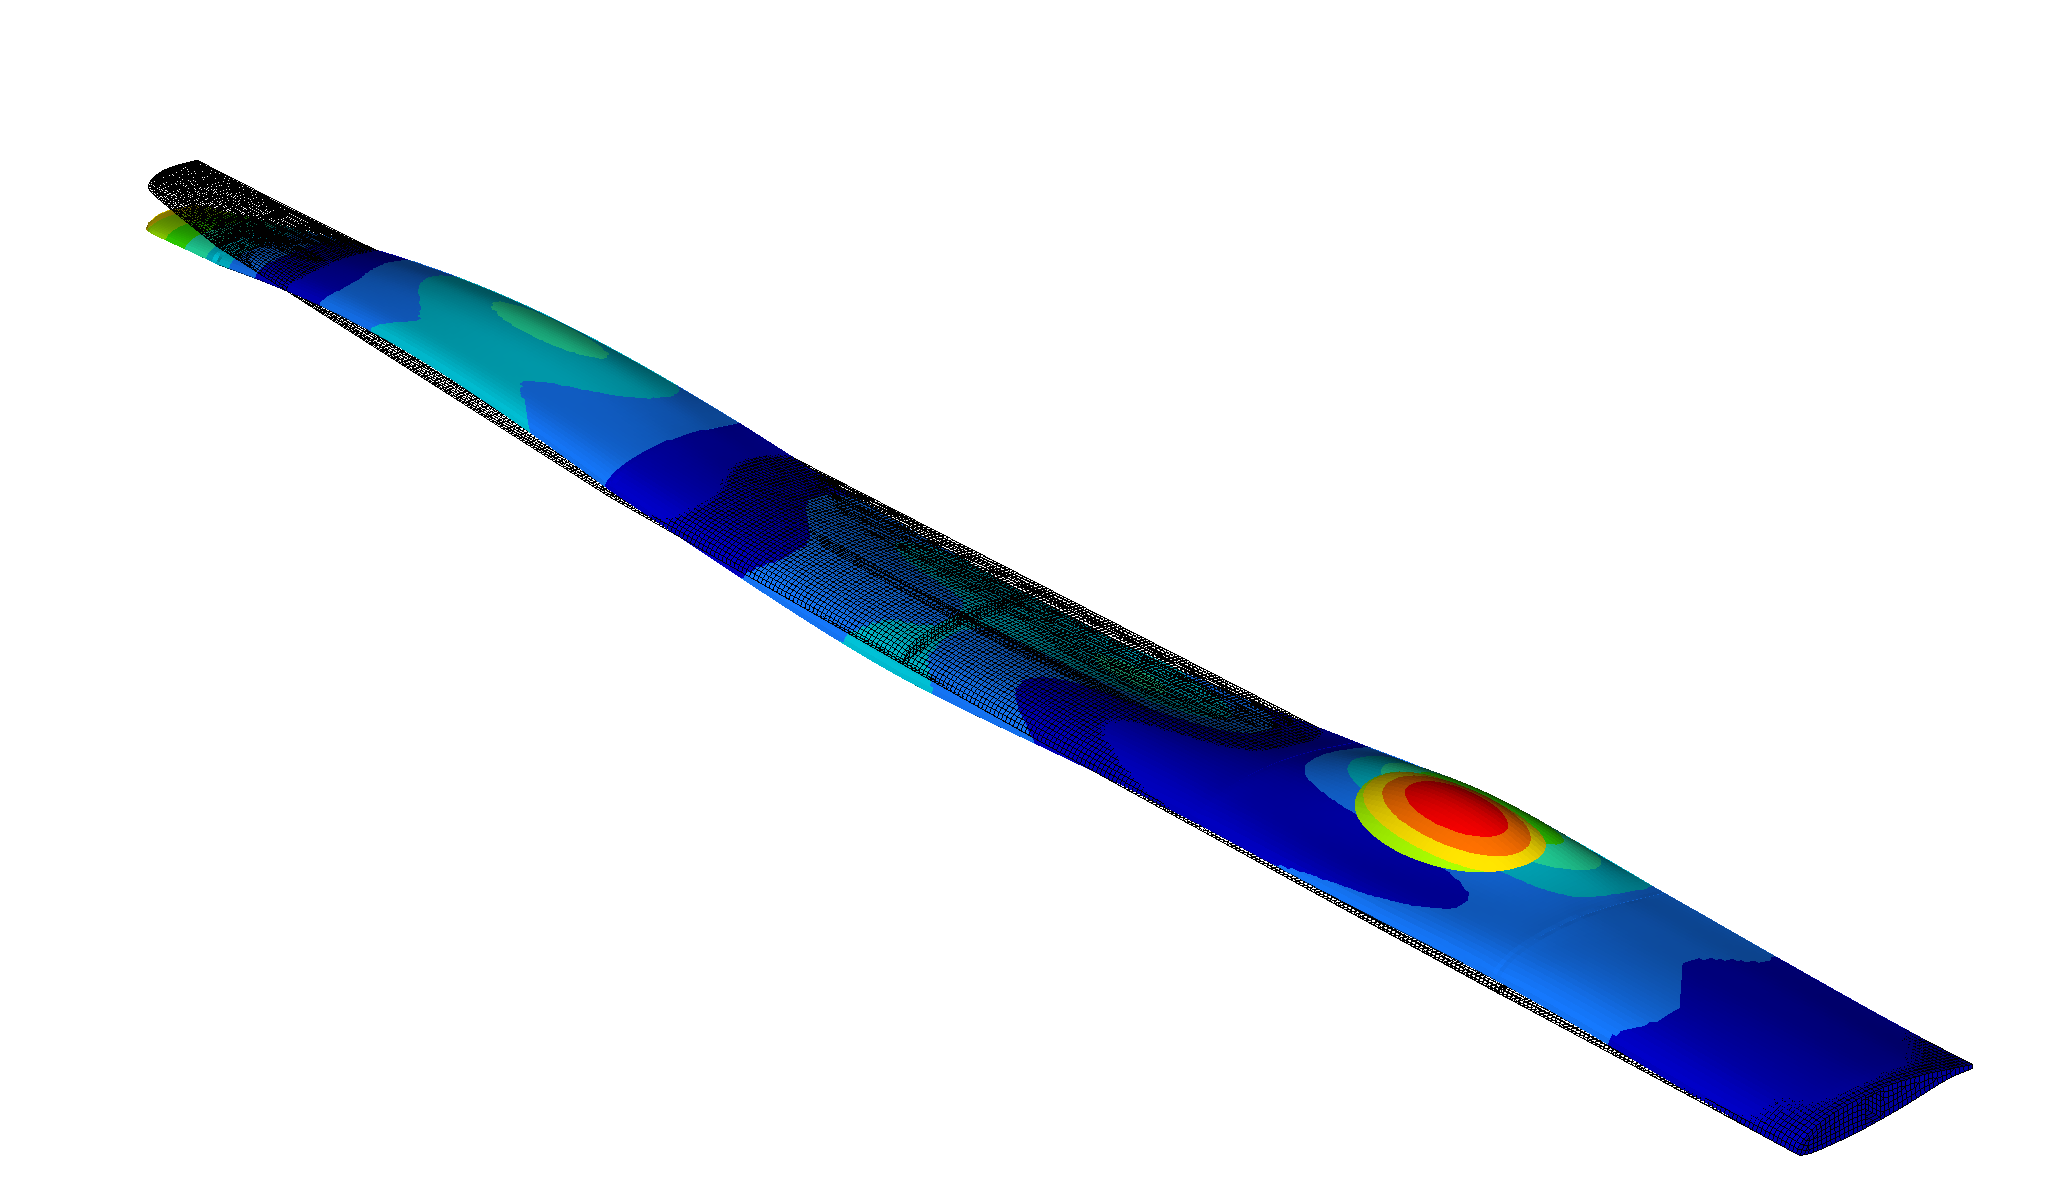
\includegraphics[width=0.5\textwidth]{mode5_30.0168Hz.png}}
  \subfloat[\textlatin{Mode 6},\quad $f = 33.99 Hz$]{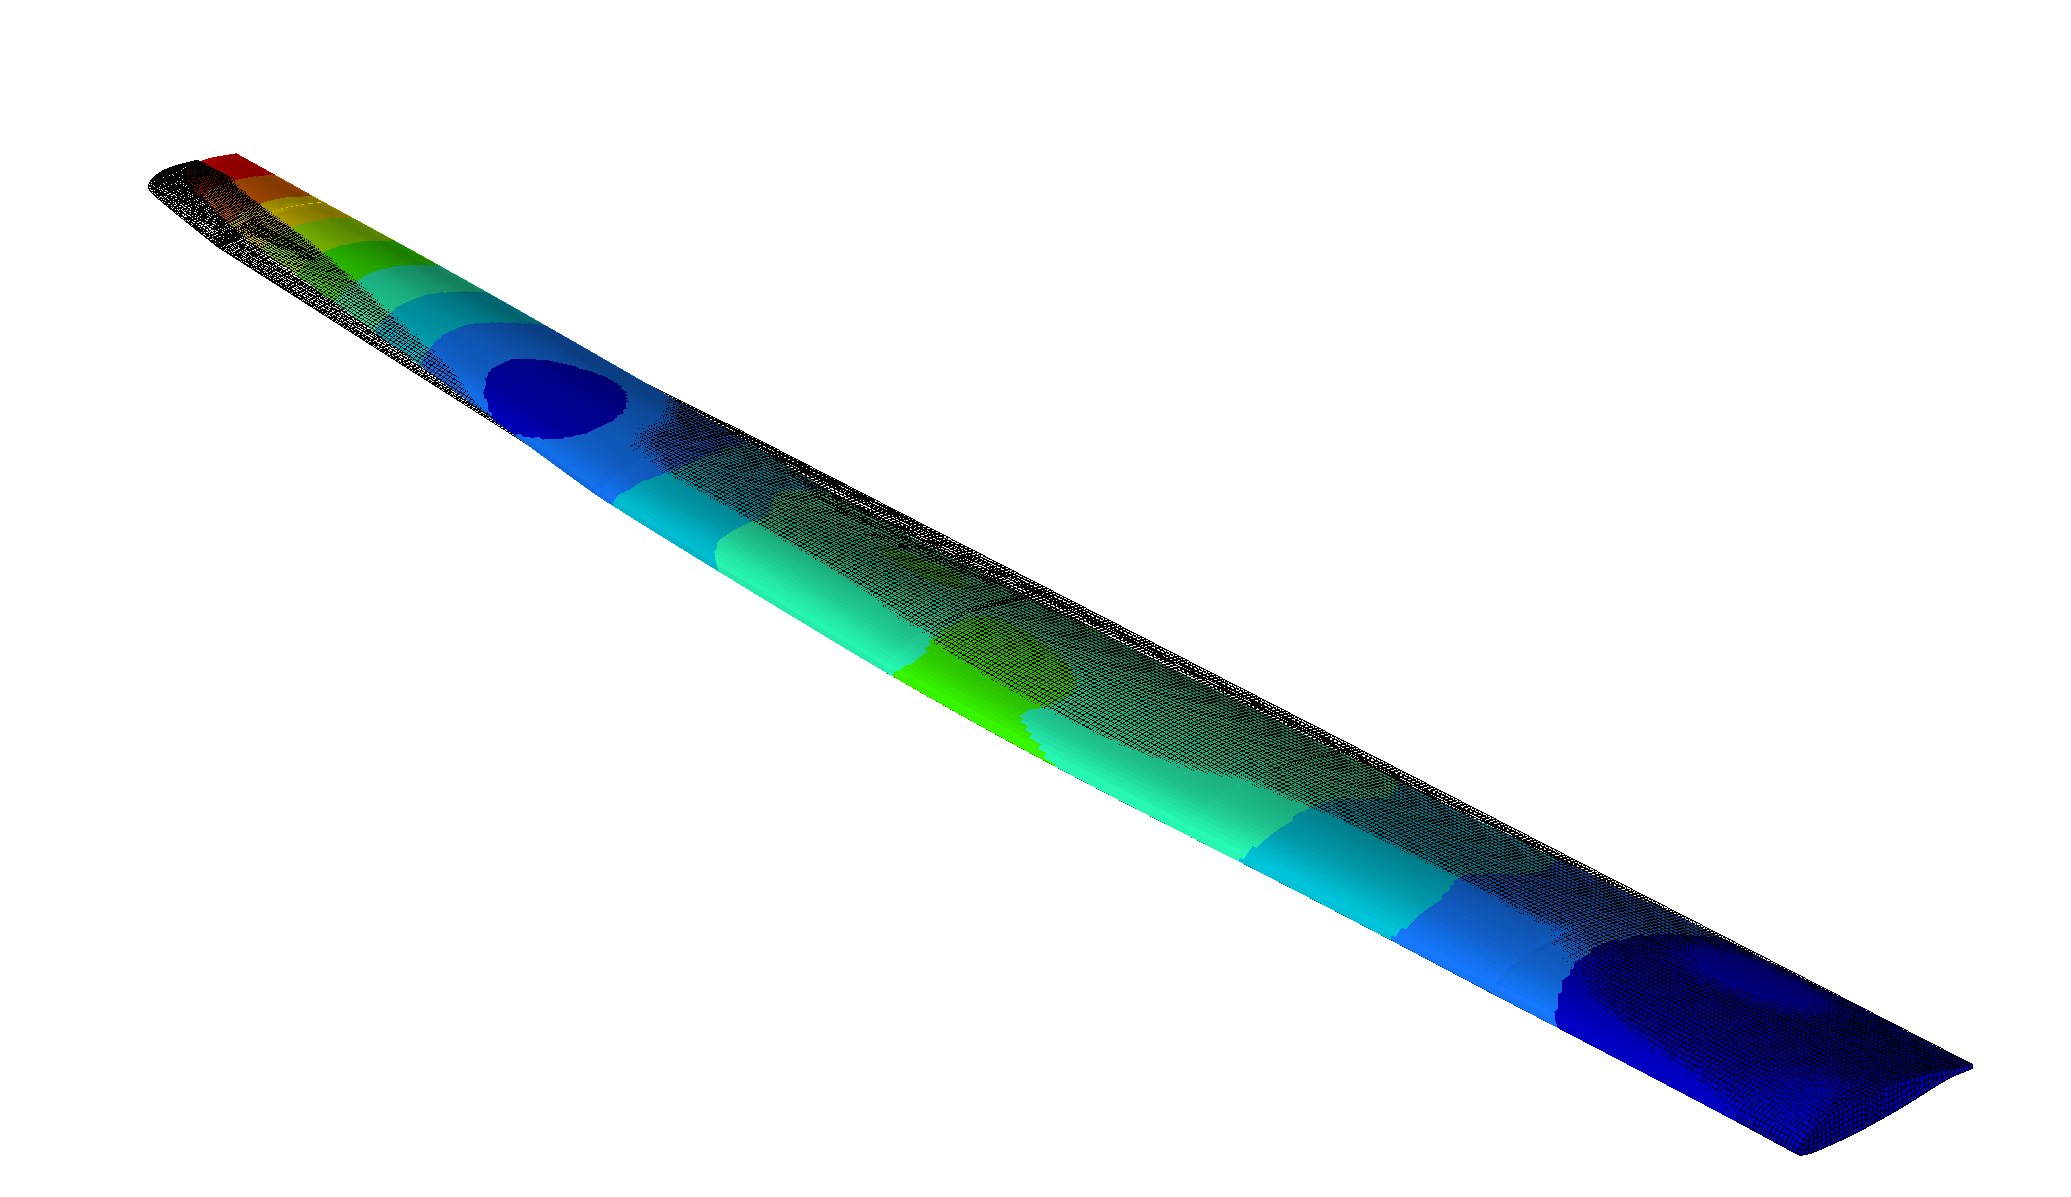
\includegraphics[width=0.5\textwidth]{mode6 33.998Hz.png}}
  \caption{Ο πρώτες 6 ιδιομορφές του φτερού \textlatin{ASW 28}}
  \label{fig:asw28modes}
\end{figure}

Από το \autoref{fig:asw28modes} μπορούν να παρατηρηθούν τα εξής:

\begin{itemize}
\item
  Η πρώτη ιδιομορφή έχει ιδιαίτερα χαμηλή ιδιοσυχνότητα, υποδεικνύοντας ότι το φτερό είναι αρκετά εύκαμπτο σε αυτήν την κατεύθυνση.
\item
  Οι ιδιομορφές 1, 2, 4 και 5 είναι όλες καμπτικές γύρω από τον άξονα $x$, 
  με αυξανόμενο αριθμό κόμβων (σταθερών σημείων) στο φτερό.

  \begin{itemize}
  \item
    Η ιδιομορφή 1 είναι η πιο απλή με ένα μόνο κόμβο στη ρίζα του φτερού. Καθώς η ιδιοσυχνότητα αυξάνεται, αυξάνεται και η πολυπλοκότητα της καμπτικής κίνησης καθώς και ο αριθμός των κόμβων.
  \item
    Η ιδιομορφή 2 έχει δύο κόμβους, ένα στη ρίζα του φτερού και έναν περίπου στα τρία τέταρτα του εκπετάσματος της πτέρυγας.
  \item
    Η ιδιομορφή 4 έχει τρεις κόμβους, ένα στη ρίζα του φτερού, ένα στη μέση και έναν περίπου στο 5/6 του εκπετάσματος της πτέρυγας.
  \item
    Η ιδιομορφή 5 έχει τέσσερις κόμβους κατανεμημένους κατά μήκος του εκπετάσματος της πτέρυγας, αλλά παρουσιάζει επίσης κάποιες ενδείξεις ταλάντωσης πλάκας στην άνω επιφάνεια της πτέρυγας, κοντά στη ρίζα, όπου τα \textlatin{ribs} είναι πιο απομακρυσμένα και υπάρχει ένα μεγάλο τμήμα επιφάνειας του φτερού χωρίς στήριξη.
  \end{itemize}
\item
  Οι ιδιομορφές 3 και 6 είναι καμπτικές γύρω από τον άξονα $z$. Η ιδιομορφή 3 έχει μόνο έναν κόμβο, ενώ η ιδιομορφή 6 έχει δύο.
\end{itemize}


\section{Αρχική Ανάλυση Πτερυγισμού}
\label{initial-flutter-analysis}

Εφαρμόζοντας στο μοντέλο τη μεθοδολογία που αναπτύχθηκε στην \autoref{asw-28-main-composite-wing-model}, προκύπτουν τα εξής αποτελέσματα:


\begin{figure}[H]
    \centering
    \includesvg[width=\textwidth]{initialFlutter.svg}
    \caption{Αρχικό διάγραμμα πτερυγισμού για τις 4 πρώτες ιδιομορφές.}
    \label{fig:initflutter}
\end{figure}


\begin{figure}[H]
    \centering
    \includesvg[width=\textwidth]{InitialFlutterMode3.svg}
    \caption{Διάγραμμα πτερυγισμού για την 3\textsuperscript{η} ιδιομορφή}
    \label{fig:initfluttermode3}
\end{figure}

Από τα Σχήματα \ref{fig:initflutter} και \ref{fig:initfluttermode3} μπορούμε να δούμε ότι το \textlatin{Flutter} συμβαίνει στην
3\textsuperscript{η} ιδιομορφή με:

\begin{equation}
V_{flutter} = 94.11\ m/s
\end{equation}

Παρατηρείται ότι η 1\textsuperscript{η} ιδιομορφή είναι πολύ πιθανό να αποκλίνει επίσης περίπου στην ίδια ταχύτητα, αν και η απόσβεσή της δεν αλλάζει πρόσημο. Η απότομη αύξηση της απόσβεσης σε μια τιμή κοντά στο μηδέν (αλλά ακόμη αρνητική), μαζί με τη μείωση της ιδιοσυχνότητας σχεδόν στο μηδέν, υποδεικνύουν την ύπαρξη στατικής αεροελαστικής απόκλισης (\textlatin{aeroelastic divergence}) που δεν καταγράφεται από τον αλγόριθμο. Η συμπεριφορά αυτή είναι αναμενόμενη για πολύ ευκαμπτες πτέρυγες με μεγάλα εκπετάσματα όταν μελετούνται με γραμμική ανάλυση πτερυγισμού, όμως όπως έχουν δείξει μελέτες μέσω μη γραμμικών προσομοιώσεων και πειραμάτων, αυτό δεν αντικατοπτρίζει κατ' ανάγκη την πραγματικότητα, διότι τα μη γραμμικά φαινόμενα υπερισχύουν σε μεγάλες μετατοπίσεις \cite{NonlinearAeroelasticStability}.

\section{Μέθοδος Βελτιστοποίησης \textlatin{Powell}}
\label{powells-optimization-method}

Μετά την εφαρμογή της μεθόδου βελτιστοποίησης \textlatin{Powell} όπως περιγράφεται στήν \autoref{applying-powells-method}, προκύπτουν τα εξής αποτελέσματα:

\subsubsection{Περίπτωση 1:}

Αυτή ήταν η πρώτη αντικειμενική συνάρτηση που διατυπώθηκε στην εξίσωση \eqref{eq:objpowell1}, καθώς ορίζει ένα πιο ολοκληρωμένο πρόβλημα βελτιστοποίησης. Η βελτιστοποίηση ολοκληρώθηκε με μερική επιτυχία. Τα αποτελέσματα παρουσιάζονται στο \autoref{fig:ValueofobjectivefunctionthroughouttheoptimizationScenario1}:

\begin{figure}[H]
    \centering
    \includesvg[width=\textwidth]{Objective1.svg}
    \caption{Τιμή της αντικειμενικής συνάρτησης κατά τη διάρκεια της βελτιστοποίησης (Περίπτωση 1)}
    \label{fig:ValueofobjectivefunctionthroughouttheoptimizationScenario1}
\end{figure}

\begin{figure}[H]
    \centering
    \includesvg[width=\textwidth]{Variables1.svg}
    \caption{Τιμή κάθε μεταβλητής βελτιστοποίησης κατά τη διάρκεια της βελτιστοποίησης (Περίπτωση 1)
    }
\end{figure}

Όπως φαίνεται ο αλγόριθμος αποτυγχάνει να βελτιώσει την αντικειμενική συνάρτηση πέρα από το αρχικό σημείο. Στην πρώτη επανάληψη, ο αλγόριθμος προσπαθεί να μειώσει τη μάζα της πτέρυγας μειώνοντας το πάχος των στρωμάτων κατά ένα δέκατο του χιλιοστού, αλλά η ταχύτητα πτερυγισμού μειώνεται υπερβολικά και επιβάλλεται η ποινή, με αποτέλεσμα μια πολύ υψηλή τιμή της αντικειμενικής συνάρτησης.

Από εκείνο το σημείο, ο αλγόριθμος πειραματίζεται με μεγαλύτερες τιμές πάχους, οι οποίες φυσικά οδηγούν σε μεγαλύτερη μάζα, αλλά με αρκετά υψηλή ταχύτητα πτερυγισμού ώστε να μην επιβληθεί η ποινή.

Τελικά, ο αλγόριθμος μειώνει το πάχος των στρωμάτων σταδιακά μέχρι να φτάσει στο αρχικό πάχος.

Ο αλγόριθμος δεν αντιλαμβάνεται ότι αλλάζοντας πρώτα τις γωνίες των στρωμάτων ώστε η ταχύτητα πτερυγισμού να αυξηθεί και στη συνέχεια μειώνοντας το πάχος, η ταχύτητα πτερυγισμού παραμένει αρκετά υψηλή ώστε να μην επιβληθεί η ποινή ενώ ταυτόχρονα μειώνεται η μάζα. Αυτή είναι μια περίπλοκη λύση, καθώς οι γωνίες δεν επηρεάζουν άμεσα τη μάζα, αλλά μόνο την ταχύτητα πτερυγισμού. Αν ο αλγόριθμος είχε εξερευνήσει καλύτερα τις γωνίες ενώ βρισκόταν στη ζώνη ποινής, θα μπορούσε να είχε αυξήσει την ταχύτητα του πτερυγισμού επαρκώς για να βγει από τη ζώνη ποινής και τελικά να βρει μια καλύτερη λύση. Δυστυχώς, αυτή η συμπεριφορά είναι αρκετά σύνθετη και ξεπερνά τις δυνατότητες αυτού του σχετικά απλού αλγορίθμου.

Τα αποτελέσματα της ανάλυσης πτερυγισμού της τελικής λύσης αυτού του αλγορίθμου παρουσιάζονται στα σχήματα \ref{fig:FlutteranalysisplotsfromPowellsmethodScenario1} και \ref{fig:Mode3FlutteranalysisPowellsmethodScenario1}:


\begin{figure}[H]
    \centering
    \includesvg[width=\textwidth]{Flutter1.svg}
    \caption{Διαγράμματα ανάλυσης πτερυγισμού από τη μέθοδο του \textlatin{Powell}. (Περίπτωση 1)}
    \label{fig:FlutteranalysisplotsfromPowellsmethodScenario1}
\end{figure}

Η πρώτη ιδιομορφή που παρουσιάζει απόκλιση είναι η ιδιομορφή 3, η οποία απεικονίζεται μόνη της στο επόμενο σχήμα ώστε να φανεί καθαρά πότε αλλάζει πρόσημο η απόσβεση.

\begin{figure}[H]
    \centering
    \includesvg[width=\textwidth]{Flutter1Mode3.svg}
    \caption{Ανάλυση πτερυγισμού της 3\textsuperscript{ης} ιδιομορφής με τη μέθοδο του \textlatin{Powell}. (Περίπτωση 1)}
    \label{fig:Mode3FlutteranalysisPowellsmethodScenario1}
\end{figure}

Η ταχύτητα με την οποία η ιδιομορφή αυτή αποκλίνει για πρώτη φορά είναι η ταχύτητα πτερυγισμού και στην προκειμένη περίπτωση:


\begin{equation}
V_{flutter} = 99.48\ m/s
\end{equation}

\subsubsection{Περίπτωση 2:}

Για να επιτευχθεί ένα καλύτερο αποτέλεσμα, χρησιμοποιείται η απλοποιημένη αντικειμενική συνάρτηση της εξίσωσης \eqref{eq:objpowell2}. 
Αυτή τη φορά, ο αλγόριθμος εξερευνά το χώρο των πιθανών λύσεων με μεγαλύτερη επιτυχία. Τα αποτελέσματα παρουσιάζονται στο \autoref{fig:objpowell2}:


\begin{figure}[H]
    \centering
    \includesvg[width=\textwidth]{Objective2.svg}
    \caption{Τιμή της αντικειμενικής συνάρτησης κατά τη διάρκεια της βελτιστοποίησης (Περίπτωση 2)}
    \label{fig:objpowell2}
\end{figure}

\begin{figure}[H]
  \centering
  \includesvg[width=\textwidth]{Variables2.svg}
  \caption{Τιμή κάθε μεταβλητής βελτιστοποίησης κατά τη διάρκεια της βελτιστοποίησης (Περίπτωση 2)}
\end{figure}

Παρατηρείται από το \autoref{fig:objpowell2} ότι η αντικειμενική συνάρτηση, η οποία τώρα αποσκοπεί στην ελαχιστοποίηση της αρνητικής ταχύτητας πτερυγισμού, έχει βελτιωθεί σημαντικά.

Επιπλέον, σύμφωνα με τον ορισμό αυτού του προβλήματος, η μεταβλητή πάχους παραμένει σταθερή και ίση με την αρχική τιμή των $0.5 mm$. Αυτό σημαίνει ότι ενώ η ταχύτητα πτερυγισμού αυξάνεται σημαντικά, η μάζα παραμένει σταθερή.

Τα διαγράμματα πτερυγισμού για την βέλτιστη λύση αυτής της μεθόδου παρουσιάζονται στα σχήματα \ref{fig:PowerllFlutterPlotScenario2} και \ref{fig:PowerllFlutter3PlotScenario2} .


\begin{figure}[H]
    \centering
    \includesvg[width=\textwidth]{Flutter2.svg}
    \caption{Διαγράμματα ανάλυσης πτερυγισμού  από τη μέθοδο του \textlatin{Powell}. (Περίπτωση 2)}
    \label{fig:PowerllFlutterPlotScenario2}
\end{figure}


\begin{figure}[H]
    \centering
    \includesvg[width=\textwidth]{Flutter2Mode3.svg}
    \caption{Ανάλυση πτερυγισμού της 3\textsuperscript{ης} ιδιομορφής με τη μέθοδο του \textlatin{Powell}. (Περίπτωση 2)}
    \label{fig:PowerllFlutter3PlotScenario2}

\end{figure}

Για άλλη μια φορά, η πρώτη ιδιομορφή που αποκλίνει είναι η ιδιομορφή 3. Αυτή τη φορά όμως, η ταχύτητα είναι πολύ μεγαλύτερη από πριν.

\begin{equation}
V_{flutter} = 175.28\ m/s
\end{equation}

Οι ιδιομορφές 1 και 4 αποκλίνουν επίσης στα $267.09$ και $177.14 m/s$ αντίστοιχα. Όπως είναι προφανές, αυτή είναι μια εξαιρετική βελτίωση της ταχύτητας πτερυγισμού του φτερού σε σχέση με την αρχική λύση, χωρίς επιπλέον υλικό και άρα με την ίδια μάζα με το αρχικό φτερό.

Το διάνυσμα που δίνει τη βέλτιστη λύση είναι:

\begin{equation}
{\vec{\mathbf{x}}}_{opt} = \lbrack 0.0005,90, - 58, - 59\rbrack^{T}
\end{equation}


\section{Βελτιστοποίηση με τη μέθοδο Γενετικών Αλγορίθμων}
\label{genetic-algorithm-optimization}

Μετά την εφαρμογή της μεθόδου γενετικών αλγορίθμων όπως περιγράφεται στήν \autoref{applying-the-genetic-algorithm}, προκύπτουν τα εξής αποτελέσματα:

\begin{figure}[H]
    \centering
    \includesvg[width=\textwidth]{fitness.svg}
    \caption{Εξέλιξη του \textlatin{fittness fucntion} της καλύτερης λύσης κάθε γενιάς κατά τη διαδικασία βελτιστοποίησης}
    \label{fig:fitnessevolution}
\end{figure}


\begin{figure}[H]
    \centering
    \includesvg[width=\textwidth]{genes.svg}
    \caption{Εξέλιξη των τιμών των γονιδίων κατά τη διάρκεια της διαδικασίας βελτιστοποίησης.}
\end{figure}



Από το \autoref{fig:fitnessevolution}, όπου απεικονίζεται η καλύτερη λύση που βρέθηκε μέχρι στιγμής σε κάθε γενιά, παρατηρείται ότι και οι δύο στόχοι βελτιώνονται μέχρι το τέλος της βελτιστοποίησης, παρόλο που αυτοί είναι αντιφατικοί μεταξύ τους. Από τα αρχεία καταγραφής της βελτιστοποίησης, η καλύτερη λύση έχει τα εξής χαρακτηριστικά:


\begin{equation}
V_{flutter} = 214.69\ m/s,\quad Mass = 45.1\ kg
\end{equation}

Οι τιμές των γονιδίων που οδηγούν στη βέλτιστη λύση είναι:


\begin{equation}
t = 0.0003\ mm,\ \ \vartheta_{1} = 43{^\circ},\ \ \vartheta_{2} = 56{^\circ},\ \ \vartheta_{3} = 76{^\circ}
\end{equation}

Το διάγραμμα πτερυγισμού  για αυτήν τη λύση παρουσιάζεται στο \autoref{fig:FlutterPlotfromGeneticAlgorithm}:

\begin{figure}[H]
    \centering
    \includesvg[width=\textwidth]{FlutterPlot4modes.svg}
    \caption{Διάγραμμα πτερυγισμού  από τον αλγόριθμο γενετικής βελτιστοποίησης.}
    \label{fig:FlutterPlotfromGeneticAlgorithm}
\end{figure}

\begin{figure}[H]
    \centering
    \includesvg[width=\textwidth]{FlutterPlotmode1.svg}
    \caption{Διάγραμμα πτερυγισμού της 1\textsuperscript{ης} ιδιομορφής από αλγόριθμο γενετικής βελτιστοποίησης}
    \label{fig:GAflutterMode1}
\end{figure}

Αν και η λύση που προκύπτει από τη μέθοδο των γενετικών αλγορίθμων φαίνεται ιδανική, εξετάζοντας το \autoref{fig:GAflutterMode1} μπορούμε να δούμε ότι πριν από την αναφερόμενη ταχύτητα πτερυγισμού των $214 m/s$, η απόσβεση  της 1\textsuperscript{ης} ιδιομορφής αλλάζει σημαντικά στα $110 m/s$ και η ιδιοσυχνότητα μειώνεται στο μηδέν, το οποίο είναι ένδειξη στατικής αεροελαστικής απόκλισης \textlatin{(static aeroelastic divergence)}. Είναι πιθανό αυτό να μη συμβαίνει στην πραγματικότητα, διότι όπως έχουμε δει σε άλλες μελέτες \cite{NonlinearAeroelasticStability}, όταν το φτερό εκτρέπεται με μεγάλες μετατοπίσεις, τα μη γραμμικά φαινόμενα γίνονται σημαντικά και απαιτούνται μη γραμμικές αναλύσεις στατικής αερολαστικότητας για τον εντοπισμό τέτοιων φαινομένων.

\section{Αποτελέσματα Πρόβλεψης μέσω Νευρωνικών Δικτύων}
\label{neural-network-prediction-results}

Σε αυτή την ενότητα, θα παρουσιαστούν τα αποτελέσματα κάθε Νευρωνικού Δικτύου που αναπτύχθηκε στήν \autoref{flutter-speed-prediction-using-neural-networks}. Παρουσιάζονται τρία βασικά διαγράμματα για την κατανόηση της απόδοσης κάθε δικτύου.

\begin{enumerate}
\def\labelenumi{\arabic{enumi}.}
\item
  Το πρώτο διάγραμμα δείχνει την τιμή της συνάρτησης απώλειας στα δεδομένα εκπαίδευσης και επικύρωσης σε κάθε εποχή της εκπαίδευσης.
\item
  Το δεύτερο διάγραμμα χρησιμοποιείται για την αξιολόγηση της απόδοσης του δικτύου με τη χρήση του διαγράμματος διασποράς \(y_{pred}\ \text{\textlatin{vs}} \ y_{true}\). Ιδανικά, αυτές οι τιμές θα ταυτίζονταν, παράγοντας μια ευθεία γραμμή με γωνία \(45{^\circ}\).
\item
  Το τρίτο διάγραμμα εμφανίζει τις διαφορές ως προς το \(y_{true}\),  \( (y_{true} - y_{pred})\ \text{\textlatin{vs}} \ y_{true} \), διευκολύνοντας την κατανόηση του μεγέθους του σφάλματος καθώς και τυχόν τάσεων που μπορεί να υπάρχουν σε συγκεκριμένες ταχύτητες πτερυγισμού.
\end{enumerate}

\subsection{Εξέταση δεδομένων εκπαίδευσης}
\label{training-data-examination}

Ένας προκαταρκτικός έλεγχος των δεδομένων πραγματοποιείται χρησιμοποιώντας ένα διάγραμμα συσχέτισης \textlatin{(pair plot)}, το οποίο είναι ένα πλέγμα γραφημάτων που επιτρέπει την οπτικοποίηση της σχέσης μεταξύ κάθε ζεύγους μεταβλητών στο σύνολο δεδομένων.


\begin{figure}[H]
    \centering
    \includesvg[width=\textwidth]{DataExploration/pairplot.svg}
    \caption{\textlatin{pair plot} των δεδομένων εκπαίδευσης}
    \label{fig:pairplot}
\end{figure}

Από το \autoref{fig:pairplot} μπορούμε να παρατηρήσουμε τις εξής σχέσεις στα συγκεντρωμένα δεδομένα:

\begin{enumerate}
\def\labelenumi{\arabic{enumi}.}
\item
  Καθώς αυξάνεται το πάχος, αυξάνεται και η προβλεπόμενη ταχύτητα πτερυγισμού.
\item
  Οι γωνίες \(\theta_{1} - \theta_{3}\) έχουν μια ισχυρά μη γραμμική συσχέτιση με την ταχύτητα πτερυγισμού χωρίς εμφανείς τάσεις.
\item
  Κατά μήκος της διαγωνίου των ιστογραμμάτων που αντιπροσωπεύουν τη συσχέτιση μιας μεταβλητής με τον εαυτό της, παρατηρείται ότι τα δεδομένα είναι κατανεμημένα τυχαία και ομοιόμορφα σε όλο το εύρος των πιθανών τιμών.
\end{enumerate}

\subsection{Νευρωνικό Δίκτυο με 1 Κρυφό Στρώμα}\label{hidden-layer-neural-network}


\begin{figure}[H]
  \centering
  \subfloat[\textlatin{training history}]{\includesvg[width=0.5\textwidth]{1HL/traininghistory.svg}} \\
  \subfloat[$Y_{true}$ \textlatin{vs} $Y_{pred}$]{\includesvg[width=0.5\textwidth]{1HL/Ytrue_vs_Ypred.svg}}
  \subfloat[\textlatin{Residuals}]{\includesvg[width=0.5\textwidth]{1HL/Residuals_vs_Ytrue.svg}}

  \caption{Απόδοση Νευρωνικου δικτύου με 1 κρυφό στρώμα}
  \label{fig:1HLNNperf}
\end{figure}

Από το \autoref{fig:1HLNNperf} καθίσταται προφανές ότι αν και αυτό το μοντέλο με μόνο ένα κρυφό στρώμα εκπαιδεύτηκε για 400 \textlatin{epochs}, οι οποίες είναι αρκετές όπως θα φανεί από τα επόμενα αποτελέσματα, το \textlatin{Mean Average Error} των δεδομένων επικύρωσης είναι πολύ μεγάλο για να είναι χρήσιμο το δίκτυο. Η διακύμανση πάνω και κάτω από τη μηδενική γραμμή στο \autoref{fig:1HLNNperf} (γ') είναι πολύ μεγάλη, με πολλά σημεία να υποεκτιμούνται ή να υπερεκτιμούνται κατά περισσότερο από $50 m/s$.


\subsection{Νευρωνικό Δίκτυο με 2 Κρυφά Στρώματα}
\label{hidden-layer-neural-network-1}
\begin{figure}[H]
  \centering
  \subfloat[\textlatin{training history}]{\includesvg[width=0.5\textwidth]{2HL/traininghistory.svg}} \\
  \subfloat[$Y_{true}$ \textlatin{vs} $Y_{pred}$]{\includesvg[width=0.5\textwidth]{2HL/Ytrue_vs_Ypred.svg}}
  \subfloat[\textlatin{Residuals}]{\includesvg[width=0.5\textwidth]{2HL/Residuals_vs_Ytrue.svg}}

  \caption{Απόδοση Νευρωνικου δικτύου με 2 κρυφά στρώματα}
  \label{fig:2HLNNperf}
\end{figure}
Αυτό το μοντέλο εκπαιδεύτηκε για 350 \textlatin{epochs}. Τα 2 κρυφά στρώματα αποδίδουν πολύ καλύτερα από ένα μόνο στρώμα. Το \textlatin{Mean Average Error} στα δεδομένα επικύρωσης στο τέλος της εκπαίδευσης είναι περίπου $7 m/s$. Το μόνο πρόβλημα είναι ότι εξακολουθεί να υπάρχει μεγάλη διακύμανση στις προβλέψεις, όπως φαίνεται από το \autoref{fig:2HLNNperf}.


\subsection{Νευρωνικό Δίκτυο με 4 Κρυφά Στρώματα}
\label{hidden-layer-neural-network-2}

\begin{figure}[H]
  \centering
  \subfloat[\textlatin{training history}]{\includesvg[width=0.5\textwidth]{4HL/traininghistory.svg}} \\
  \subfloat[$Y_{true}$ \textlatin{vs} $Y_{pred}$]{\includesvg[width=0.5\textwidth]{4HL/Ytrue_vs_Ypred.svg}}
  \subfloat[\textlatin{Residuals}]{\includesvg[width=0.5\textwidth]{4HL/Residuals_vs_Ytrue.svg}}

  \caption{Απόδοση Νευρωνικου δικτύου με 4 κρυφά στρώματα}
  \label{fig:4HLNNperf}
\end{figure}

Το νευρωνικό δίκτυο με τέσσερα κρυφά στρώματα εκπαιδεύτηκε για 300 \textlatin{epochs}, διότι το \textlatin{validation loss} αρχίζει να εξομαλύνεται, όπως φαίνεται από το \autoref{fig:4HLNNperf} (α'). Η κατανομή των δεδομένων γύρω από τη γραμμή μηδενικής διαφοράς δεν είναι πολύ πιο στενή σε σχέση με το προηγούμενο μοντέλο, όπως φαίνεται στο \autoref{fig:4HLNNperf} (γ').


\subsection{Νευρωνικό Δίκτυο με 6 Κρυφά Στρώματα}
\label{hidden-layer-neural-network-3}

\begin{figure}[H]
  \centering
  \subfloat[\textlatin{training history}]{\includesvg[width=0.5\textwidth]{6HL/traininghistory.svg}} \\
  \subfloat[$Y_{true}$ \textlatin{vs} $Y_{pred}$]{\includesvg[width=0.5\textwidth]{6HL/Ytrue_vs_Ypred.svg}}
  \subfloat[\textlatin{Residuals}]{\includesvg[width=0.5\textwidth]{6HL/Residuals_vs_Ytrue.svg}}

  \caption{Απόδοση Νευρωνικου δικτύου με 6 κρυφά στρώματα}
  \label{fig:6HLNNperf}
\end{figure}

Το νευρωνικό δίκτυο με 6 κρυφά στρώματα εκπαιδεύτηκε για 250 \textlatin{epochs} για να αποφευχθεί η υπερεκπαίδευση (\textlatin{overfitting}), καθώς η απώλεια επικύρωσης παραμένει στάσιμη μετά την εποχή 220. Αυτό φαίνεται στο \autoref{fig:6HLNNperf}.

Η κατανομή των \textlatin{resuduals} είναι καλύτερη αλλά εξακολουθεί να είναι υψηλή, αν και βελτιώνεται σε σχέση με το προηγούμενο μοντέλο, όπως φαίνεται στο Σχήμα \autoref{fig:6HLNNperf} (γ').

\subsection{Νευρωνικό Δίκτυο με Ρυθμισμένες Υπερπαραμέτρους}
\label{hyperparameter-tuned-neural-network}

Οι υπερπαράμετροι που επιλέχθηκαν από τον αλγόριθμο \textlatin{HyperBand}, ο οποίος περιγράφηκε στην \autoref{flutter-speed-prediction-using-neural-networks}, είναι οι εξής:

\begin{itemize}
\item
  Αριθμός κρυφών στρωμάτων: 5.
\item
  Αριθμός νευρώνων για κάθε στρώμα:
  \(1024,\ \ 512,\ \ 256,\ \ 512,\ \text{και}\ 1024\) αντίστοιχα
\item
  Συνάρτηση ενεργοποίησης για κάθε στρώμα: \textlatin{ReLu}.
\item
  Ρυθμός μάθησης του \textlatin{Adam Optimizer}: $0.001$.
\end{itemize}

Η προκύπτουσα δομή του μοντέλου μπορεί να φανεί στο \autoref{fig:HypertunedStructure}.

\begin{figure}
  \centering
  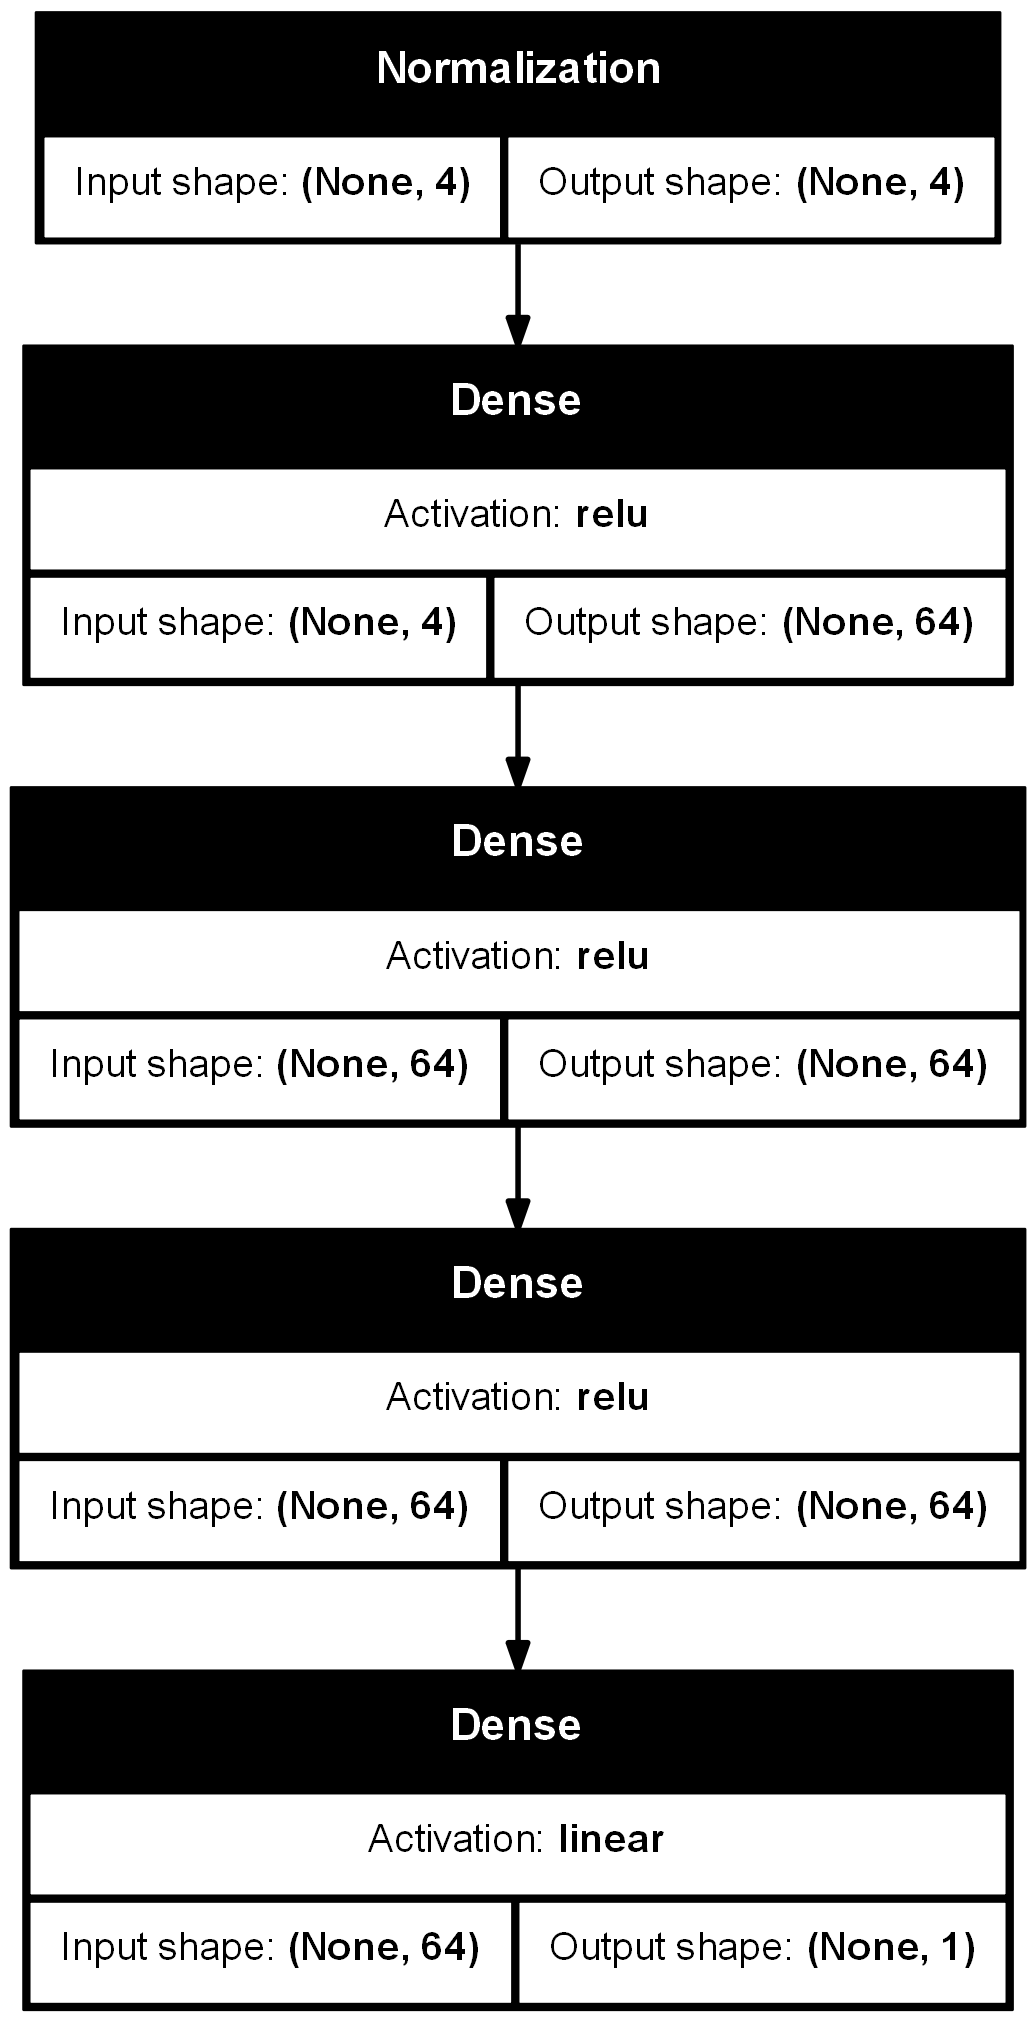
\includegraphics[width=0.38\textwidth]{tunedmodel_24_09_2024/structure.png} 
  \caption{Δομή βελτιστοποιημένου Νευρωνικού Δικτύου.}
  \label{fig:HypertunedStructure}
\end{figure}


\begin{figure}[H]
  \centering
  \subfloat[\textlatin{training history}]{\includesvg[width=0.5\textwidth]{tunedmodel_24_09_2024/traininghistory.svg}} \\
  \subfloat[$Y_{true}$ \textlatin{vs} $Y_{pred}$]{\includesvg[width=0.5\textwidth]{tunedmodel_24_09_2024/Ytrue_vs_Ypred.svg}}
  \subfloat[\textlatin{Residuals}]{\includesvg[width=0.5\textwidth]{tunedmodel_24_09_2024/Residuals_vs_Ytrue.svg}}

\caption{Απόδοση \textlatin{Hyperparameter tuned} Νευρωνικού δικτύου}
  \label{fig:HypertunedNNperf}
\end{figure}

Όπως φαίνεται από το \autoref{fig:HypertunedNNperf}, αυτό το μοντέλο εκπαιδεύτηκε για 200 \textlatin{epochs}, καθώς το MAE επικύρωσης σταματά να μειώνεται μετά από αυτό το σημείο. Αυτό το μοντέλο παρουσιάζει το χαμηλότερο MAE από όλα τα υπόλοιπα μοντέλα, με \(MAE < 5 m/s\) στην επικύρωση.

Επιπλέον, η κατανομή των δεδομένων γύρω από τη Γραμμή Μηδενικής Διαφοράς στο \autoref{fig:HypertunedNNperf} (γ'), είναι η πιο στενή από όλα τα μοντέλα, παράγοντας έτσι τα καλύτερα αποτελέσματα μέχρι στιγμής. Αξιοσημείωτο είναι επίσης ότι αυτό το μοντέλο έχει τον υψηλότερο αριθμό παραμέτρων που μπορούν να εκπαιδευτούν και απαιτεί τον περισσότερο χρόνο εκπαίδευσης.

